\RequirePackage{luatex85}
\PassOptionsToPackage{shorthands=off}{babel}
\makeatletter
\disable@package@load{fontenc}
\makeatother
\let\oldlooseness=\looseness
\documentclass{csbulletin}
\setcounter{secnumdepth}{3}
\usepackage{luavlna, float}
\usepackage[strict]{lua-widow-control}

\usepackage{minted}
\usemintedstyle{bw}
% \setminted{firstnumber=last, linenos}
\newenvironment{mintedblock}{%
  \par\vspace{\topsep}\vspace{\partopsep}%
  \begingroup
  \fvset{listparameters=\setlength{\topsep}{0pt}\setlength{\partopsep}{0pt}}%
}{%
  \endgroup
  \par\vspace{\topsep}\vspace{\partopsep}%
}

\usepackage{csquotes}
\usepackage[
  backend=biber,
  style=iso-numeric,
  citestyle=numeric-comp,
  sortlocale=cs,
  autolang=other,
  bibencoding=UTF8,
  mincitenames=2,
  maxcitenames=2,
]{biblatex}
\addbibresource{main.bib}
\renewcommand\multicitedelim{\addsemicolon\space}

\usepackage{sideways-figure, graphicx, afterpage, subcaption, tikz}
\graphicspath{{./images/}}
\usetikzlibrary{arrows.meta}

\usepackage[
  implicit=false,
  hidelinks,
]{hyperref}
\newcommand\vref[1]{\ref{#1} na straně~\pageref{#1}}

\newcommand\pkg{\textsf}
\ExplSyntaxOn
\newcommand
  \acro
  [ 1 ]
  {
    \tl_set:Nn
      \l_tmpa_tl
      { #1 }
    \regex_replace_all:nnN
      { [^\d]+ }
      { \c{textsc} \cB\{ \c{MakeLowercase} \cB\{ \0 \cE\} \cE\} }
      \l_tmpa_tl
    \regex_replace_all:nnN
      { \d+ }
      { \c{oldstylenums} \cB\{ \0 \cE\} }
      \l_tmpa_tl
    \tl_use:N
      \l_tmpa_tl
  }
\ExplSyntaxOff

\begin{document}

\title{Příprava videozáznamu české premiéry multimediálního díla ,,Fantasia Apocalyptica``}
\EnglishTitle{Recording the Czech premiere of the ``Fantasia Apocalyptica'' multimedia work}
\author{Vít Starý Novotný}
\podpis{Vít Starý Novotný, witiko@mail.muni.cz}
\maketitle[1.5ex]

\selectlanguage{czech}
\singlechars{czech}{AaIiVvOoUuSsZzKk}

\begin{abstract}
11. října 2019 se při příležitosti oslav 25. výročí založení Fakulty informatiky Masarykovy univerzity uskutečnila česká premiéra multimediálního díla \emph{Fantasia Apocalyptica} za osobní účasti autora, Donalda Knutha. Z představení byl pořízen videozáznam, který je veřejně dostupný na YouTube kanálu Fakulty informatiky.

V tomto článku popisuji přípravu záznamu od akvizice a zpracování surových audiovizuálních dat přes přípravu replik panelů doprovázejících představení po spojení jednotlivých částí do výsledného záznamu. S výjimkou střihu úvodního slova a závěru a navýšení rozlišení videa proběhlo veškeré zpracování pomocí svobodných nástrojů jako \TeX, Audacity, FFmpeg, \acro{MLT} a ImageMagick. V článku ukazuji, jak může čtenář tyto nástroje použít při přípravě vlastních záznamů.
\end{abstract}
\klicovaslova: audiovizuální záznam, zpracování videa, titulky, zpracování zvuku, kinetická typografie, \TeX, Audacity, FFmpeg, \acro{MLT}, ImageMagick, waifu2x, \acro{ASS}

\bigskip

11. října 2019 se v jezuitském kostele Nanebevzetí Panny Marie uskutečnila česká premiéra multimediálního díla \emph{Fantasia Apocalyptica}~\cite{knuth2023fantasia} za osobní účasti autora, Donalda Knutha. Z představení byl pořízen videozáznam, který je veřejně dostupný na YouTube kanálu Fakulty informatiky Masarykovy univerzity~(\acro{FI~MU})~\cite{fimu2020czech}. Předchozí články ve Zpravodaji \CSTUG u popisují průběh představení~\cite{luptak2019fantasia} a přednášek Donalda Knutha při příležitosti návštěvy Brna~\cite{szaniszlo2020dva}. V tomto článku popisuji přípravu záznamu představení.

Nejprve v sekci~\ref{sec:akvizice} popisuji akvizici a zpracování surových audiovizuálních dat. Následně v sekci~\vref{sec:uvodni-slovo-a-zaver} popisuji přípravu videozáznamu úvodního slova a závěru představení. Dále v sekci~\vref{sec:panely} popisuji přípravu panelů doprovázejících představení. Nakonec v sekci~\vref{sec:spojeni} popisuji spojení jednotlivých částí do výsledného záznamu. V sekci \vref{sec:zaver} shrnuji poznatky z článku a popisuji promítání hotového videozáznamu na \acro{FI~MU} 18. prosince 2019.

\section{Akvizice a zpracování videa a zvuku}
\label{sec:akvizice}
Video a zvuk představení zaznamenali a předzpracovali Petr Šiler, Petr „Tudy“ Holubář a studenti z laboratoře \acro{LEMMA}~\cite{LEMMA}. Následně jsem u videa sjednotil formát dat a do zvuku představení jsem přimíchal zvuky okolí a úvodní slovo Jiřího Zlatušky.

\subsection{Záznam videa}
Video představení zaznamenal Pavel Šiler na kameru Sony~\acro{PXW-X70}. Video zahrnuje přednášky Donalda Knutha na \acro{FI MU}~\autocites{2019-10-08-video-Knuth-QA1-Sony-Siler}{2019-10-09-video-Knuth-QA2-Sony-Siler}[adresář~\texttt{staticka/}]{2019-10-11-video-Fantasia-apocalyptica-Sony-Siler}, záběry kostela a varhan a úvodní slovo Jiřího Zlatušky.

\vspace{-10pt}
\subsection{Zpracování videa}
Ačkoliv jsem video obdržel v rozlišení $1920\times1080$\,px a s frekvencí 25 snímků za vteřinu, od výsledného videozáznamu se očekávalo alespoň dvojnásobné rozlišení \acro{4K} a frekvence 50 snímků za vteřinu.
Zatímco záznamy přednášek jsem obdržel v prokládaném (tzv. ,,interlaced``) formátu, záběry kostela, varhan a úvodní slovo jsem obdržel v neprokládaném (tzv. ,,progressive``) formátu. Zatímco záznamy přednášek a úvodní slovo byly zabírány ze stativu, záběry kostela a varhan byly pořízeny z ruky. Cílem zpracování videa bylo nejen navýšení rozlišení a snímkové frekvence, ale i sjednocení formátu videa a stabilizace záběrů z ruky.

Video jsem zpracoval svobodným nástrojem FFmpeg~\cite{ffmpeg} a otevřeným nástrojem waifu2x~\cite{waifu2x}, vizte obrázky~\ref{fig:ffmpeg-waifu2x} a~\ref{fig:minterpolate-yadif}. Nejprve jsem stabilizoval záběry z ruky filtry \texttt{vidstabdetect}~\cite{vidstabdetect} a~\texttt{vidstab\discretionary{\textrm{-}}{}{}transform}~\cite{vidstabtransform} nástroje FFmpeg. Následně jsem navýšil rozlišení a snímkovou frekvenci následně:
\begin{itemize}
\item U neprokládaných videí jsem nejprve navýšil rozlišení nástrojem waifu2x. Následně jsem navýšil snímkovou frekvenci filtrem \texttt{minterpolate}~\cite{minterpolate} nástroje FFmpeg, který chybějící snímky interpoluje podle okolních snímků.
\item U prokládaných videí jsem nejprve navýšil snímkovou frekvenci filtrem \texttt{yadif}~\cite{yadif}, který chybějící půlsnímky interpuje podle okolních půlsnímků a řádků. Následně jsem navýšil rozlišení nástrojem waifu2x.
\end{itemize}

\begin{figure}[b!]
\vspace{-10pt}
\input images/ffmpeg
\caption{Diagram aktivit zpracování videa pomocí nástrojů FFmpeg a waifu2x.}
\label{fig:ffmpeg-waifu2x}
\end{figure}

\begin{figure}[H]
\input images/minterpolate-yadif
\caption{Navýšení snímkové frekvence videa pomocí filtrů nástroje FFmpeg.}
\label{fig:minterpolate-yadif}
\end{figure}%
\begin{filecontents}[overwrite,nosearch,noheader]{example-minterpolate-frames-01.sh}
$ ffmpeg -i vstupní-video.mp4 -vf minterpolate obrázky-snímků/%06d.png
\end{filecontents}
\begin{filecontents}[overwrite,nosearch,noheader]{example-minterpolate-frames-02.sh}
$ ffmpeg -framerate 50 obrázky-snímků/%06d.png výstupní-video.mp4
\end{filecontents}
\footnotetext{Při rychlém pohybu kamery nebo zabíraného objektu mohou při použití filtru \texttt{minterpolate} vznikat vizuální artefakty, především na okrajích snímků a objektů. Při zpracování přednášek Donalda Knutha na \acro{FI MU} jsem proto ze vstupního videa nejprve vytvořil obrázky snímků:
\begin{mintedblock}
\inputminted{bash}{example-minterpolate-frames-01.sh}
\end{mintedblock}
\noindent
Následně jsem obrázky snímků ručně prošel a smazal jsem ty, na kterých byly viditelné artefakty na osobě Donalda Knutha. Nakonec jsem z obrázků snímků vytvořil výsledné video:
\begin{mintedblock}
\inputminted{bash}{example-minterpolate-frames-02.sh}
\end{mintedblock}
\noindent
Video mělo proměnlivou frekvenci 25--50 snímků za vteřinu podle počtu smazaných obrázků snímků v dané části videa.}

% TODO: Přidat ilustraci superrozlišení nástroje waifu2x:
% - https://is.muni.cz/el/fi/podzim2020/PV212/index.qwarp?prejit=5595949
% - https://nlp.fi.muni.cz/raslan/2021/paper4.pdf

\subsection{Záznam zvuku}
Zvuk představení byl zaznamenán šesti mikrofony:
\begin{itemize}
    \item \textls[-2]{Dva mikrofony Zoom \acro{H1}~\cite{2019-10-11-audio-Fantasia-apocalyptica-ZoomH1-TS} byly umístěny na řečnickém pultu a nad panely.}
    \item Dva mikrofony Oktava~\acro{MK012}~\cite[soubor~\texttt{ORTF-MK012\_nearReversed.flac}]{2019-10-11-audio-Fantasia-apocalyptica-Mix-Tudio} byly umístěny na kůru a namířeny do kostela.
    \item Mikrofon Roland~\acro{R26}~\cite{2019-10-11-audio-Fantasia-apocalyptica-RolandR26zLemma-organ} a mikrofon kamery Sony~\acro{PXW-X70}~\cite{2019-10-11-audio-Fantasia-apocalyptica-Sony-Siler} byly umístěny na kůru a namířeny na varhany.
\end{itemize}

Zvuk předzpracoval Petr „Tudy“ Holubář~\cite{2019-10-11-audio-Fantasia-apocalyptica-Mix-Tudio}. Hlavním vstupem jeho mixu byl prostorový záznam z mikrofonů Oktava~\acro{MK012}, do kterého pro konkrétnost lehce přimíchal přímý záznam varhan z mikrofonu Roland~\acro{R26}. Pro zúžení dynamického rozsahu použil Petr analogový kompresor Hammerwave.

\subsection{Zpracování zvuku}
Zvuk jsem zpracoval svobodným programem Audacity~\cite{2019-11-19-audio-Fantasia-apocalyptica-Mix-Novotny,2019-12-09-audio-Fantasia-apocalyptica-Mix-Novotny}, vizte Obrázek~\ref{fig:audacity}.%
\begin{sideways-figure}{fig:audacity}
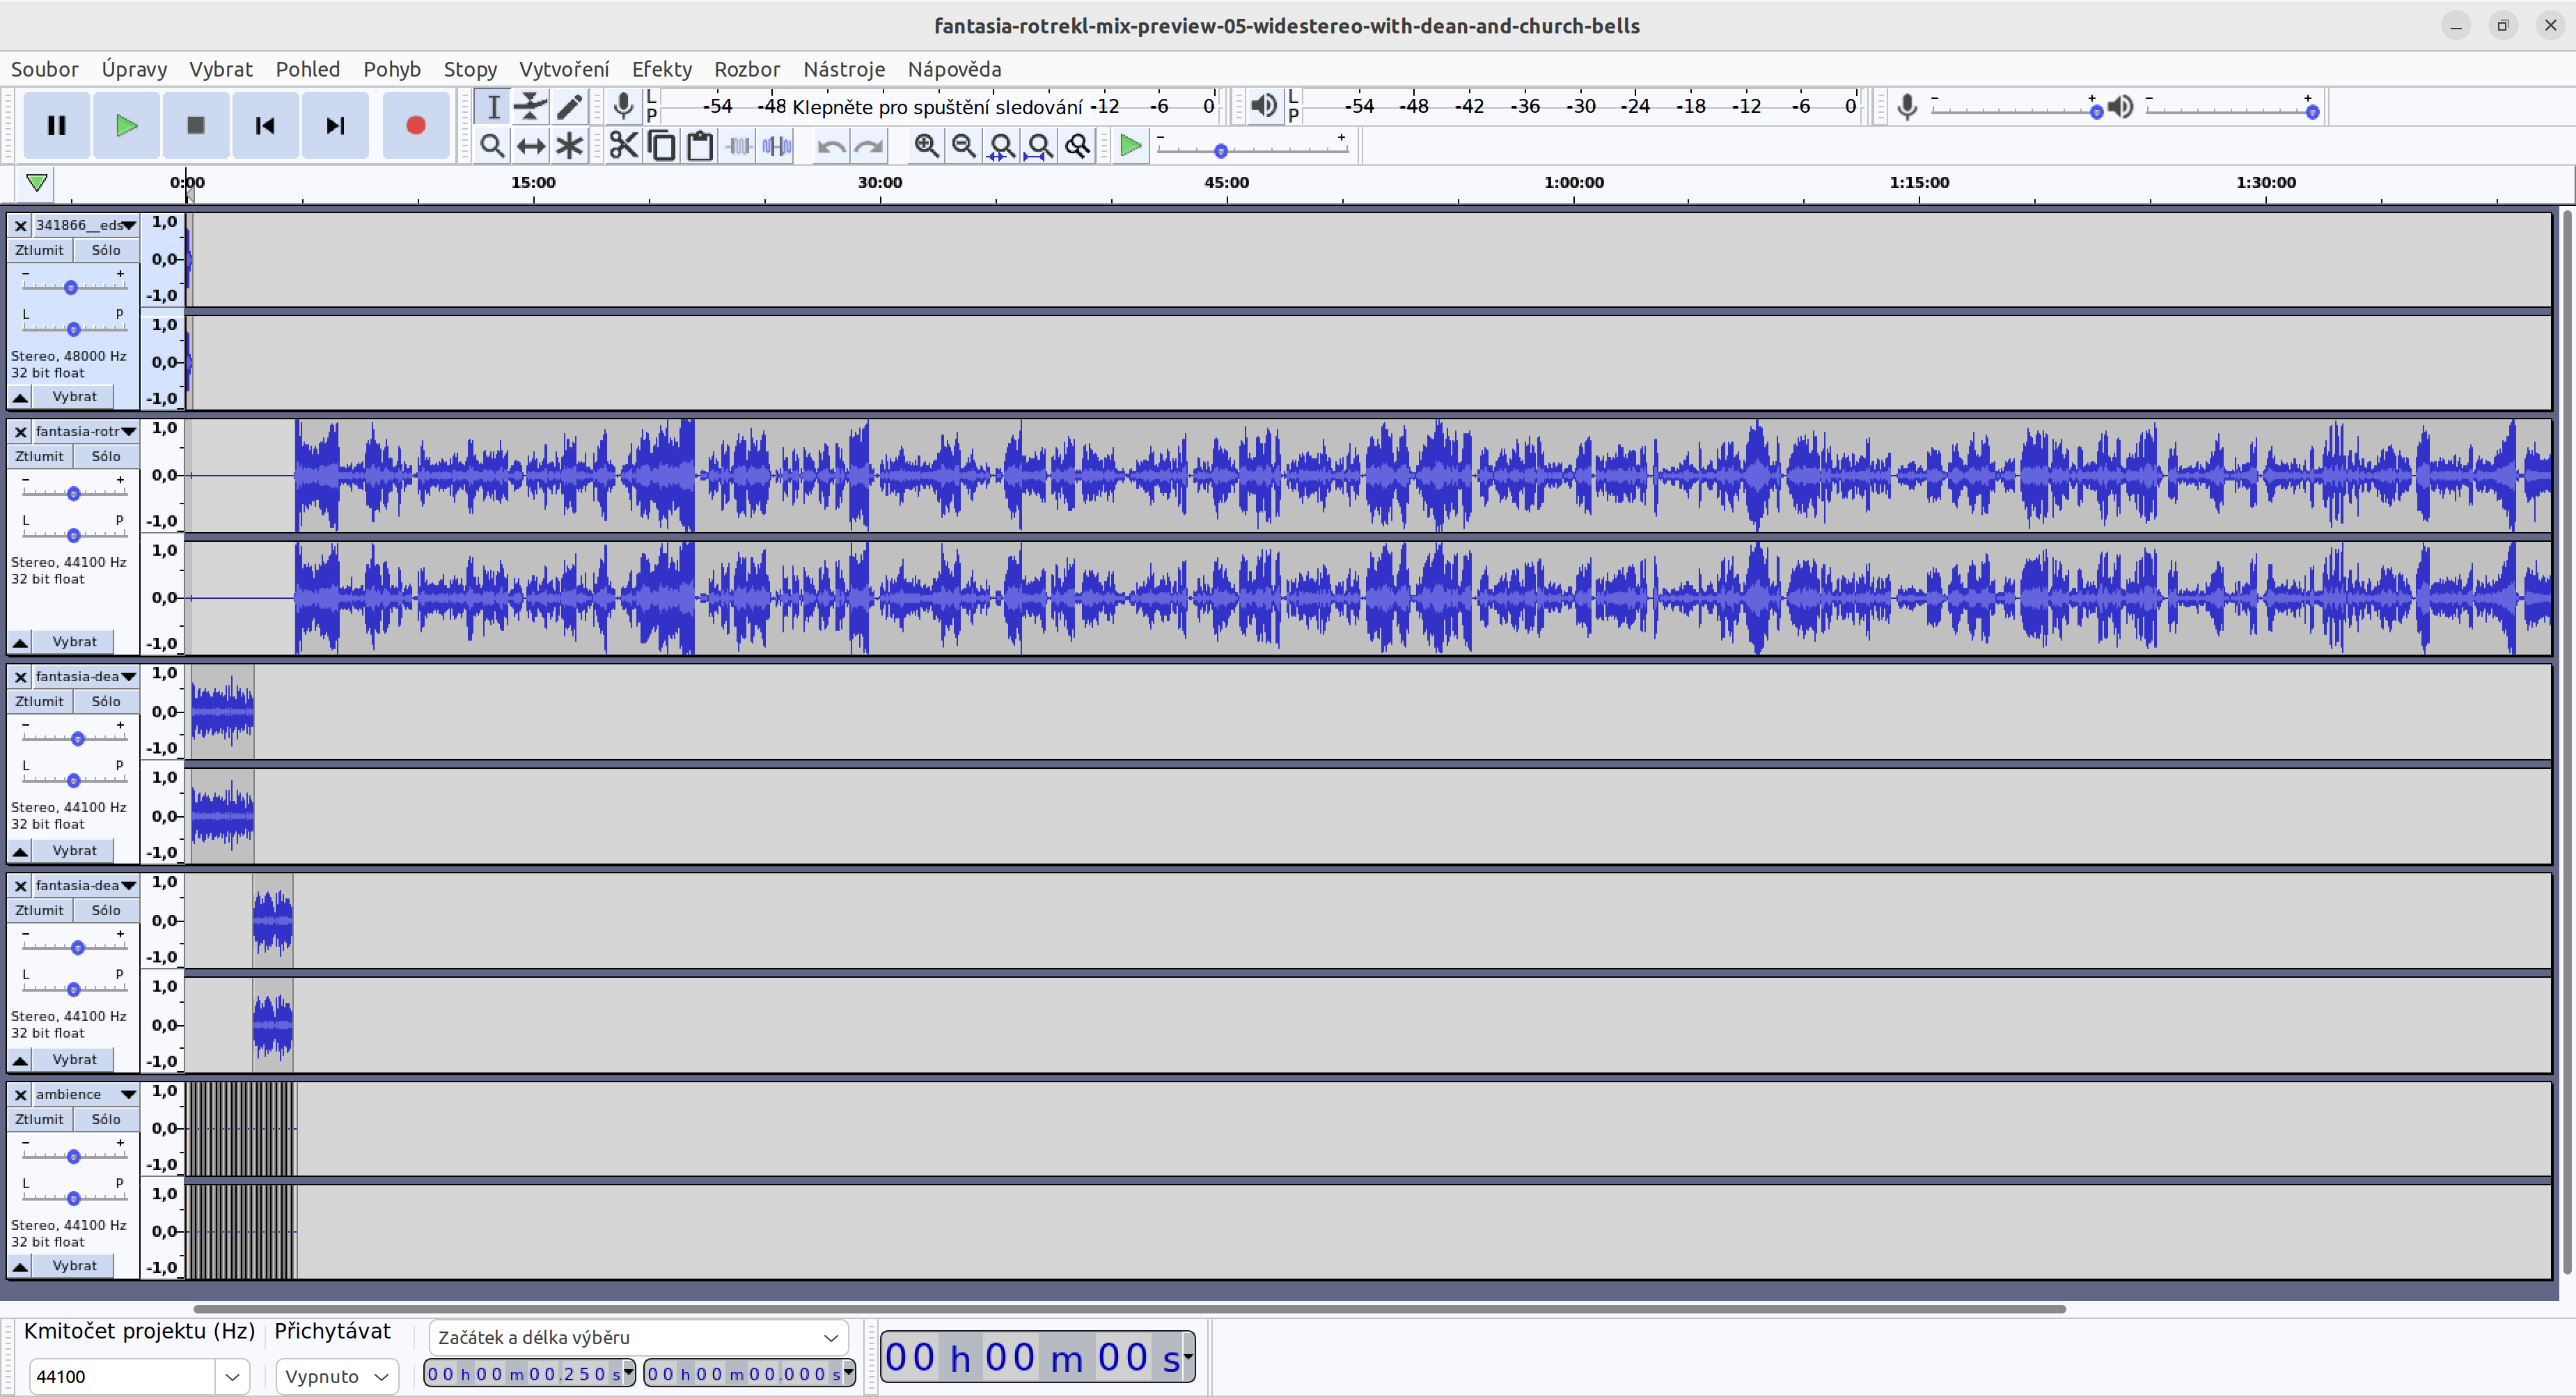
\includegraphics[width=\linewidth]{audacity}
\caption{Zpracování zvuku ve svobodném programu Audacity. Výsledný mix zahrnuje zvuk zvonu (nahoře), předzpracovaný zvuk představení od Petra „Tudy“ Holubáře (druhý odshora) a úvodní slovo Jiřího Zlatušky (uprostřed) podkreslené zvuky okolí (dole).}
\end{sideways-figure}
Výsledný mix zahrnuje svobodný zvuk zvonu kostnické katedrály~\cite{edsward2016church}, předzpracovaný zvuk představení od Petra Holubáře a úvodní slovo Jiřího Zlatušky podkreslený zvuky okolí z mikrofonů Oktava~\acro{MK012}.

\section{Příprava videozáznamu úvodního slova a závěru}
\label{sec:uvodni-slovo-a-zaver}
TODO

\subsection{Střih úvodního slova a závěru}
TODO

\subsection{Titulky úvodního slova}
TODO

\section{Příprava panelů doprovázejících varhanní oratorium}
\label{sec:panely}
TODO

\subsection{Příprava panelu s trojjazyčným textem Zjevení Janova}
TODO

\subsection{Příprava panelu s ilustracemi Duanea Bibbyho}
TODO

\subsection{Příprava panelu s notami pro varhany}
TODO

\section{Spojení jednotlivých částí do výsledného videa}
\label{sec:spojeni}
TODO

\section{Závěr}
\label{sec:zaver}
TODO

\begingroup
\sloppy
\printbibliography
\endgroup

\begin{summary}
On October 11, 2019, the Czech premiere of \emph{Fantasia Apocalyptica} was held for the 25th anniversary of Masaryk University's Faculty of Informatics, featuring its author, Donald Knuth. A video recording of the perfomance was taken and published at the YouTube channel of the Faculty of Informatics.

In this article, I describe how the recording was prepared from processing the raw footage through replicating the panels that accompanied the performance to the final composition. Apart from super-resolution imaging and the editing of the intro and the wrap-up, only free open-source tools like \TeX, Audacity, FFmpeg, \acro{MLT}, and ImageMagick were used. In the article, I describe how readers can use these tools to create their own recordings.

\keywords: footage acquisition, audio-visual production, subtitles, kinetic typography, \TeX, Audacity, FFmpeg, \acro{MLT}, ImageMagick, waifu2x, \acro{ASS}
\end{summary}

\end{document}